\section{Model selection with stochastic block models}
\label{sec:ch7:modelselect}

In Section \ref{sec:ch7:comm_detect} and Section \ref{sec:ch7:testing}, we covered a lot of ground for block models. In Section \ref{sec:ch5:psd_block}, you learned many separate models that you can use to describe $2 \times 2$ random networks with block structures. Many of these models, in fact, could be thought of as \textit{generalizations} of other models, in that some of the models you learned about could describe others of the models, but not necessarily the other way around. 

Let's imagine that you have a network sample, and that you were given (or learned through community detection) a set of community assignments for each node. In the below code, we'll take a look at a network sample from a $SBM_n(\vec z, B)$ random network with a homophilic block matrix:

\begin{lstlisting}[style=python]
import numpy as np
from graspologic.simulations import sbm


nk = 50  # 50 nodes per community
K = 2  # the number of communities
n = nk * K  # total number of nodes

zs = np.array([k for k in range(1, K + 1) for i in range(nk)])
# block matrix
B = np.array([[0.6, 0.3],[0.3, 0.5]])
# generate network sample
A = sbm([nk, nk], B)
\end{lstlisting}

A plot of the true underlying block matrix is shown in Figure \ref{fig:ch7:model:ex}(A), and the adjacency matrix is shown in Figure \ref{fig:ch7:model:ex}(B).

From what we learned in Section \ref{sec:ch6:mle}, given a network and a set of community assignments, a logical step to learn more about your network is to estimate the block probability matrix. We can do this using the below code:

\begin{lstlisting}[style=python]
from graspologic.models import SBMEstimator

# instantiate the class object and fit
model = SBMEstimator(directed=False, loops=False)
model.fit(A, y=zs)
# obtain the estimate of the block matrix
Bhat = model.block_p_
\end{lstlisting}

The estimated block matrix is shown in Figure \ref{fig:ch7:model:ex}(C). As you can see, the estimated probabilities look to largely support a homophilic structure: the two on-diagonal entries exceed the estimated off-diagonal entries. 

However, there's a problem: remember in Section \ref{sec:ch7:testing}, a key focus that we had was determining when differences between estimated probabilities indicated that the true underlying probabilities differed. We learned that, even though two probability estimates might be different, we leverage statistical strategies to determine whether these differences are more, or less, than we would expect given natural variation that can arise in the data. When the observed differences are less than we would expect with natural variability, we determined that we tended to favor reporting that we did not have evidence to reject the null hypothesis. When the observed differences exceed what we would expect with natural variability, we determined that we tended to favor reporting that the data supported rejecting the null hypothesis.

\begin{figure}[h]
    \centering
    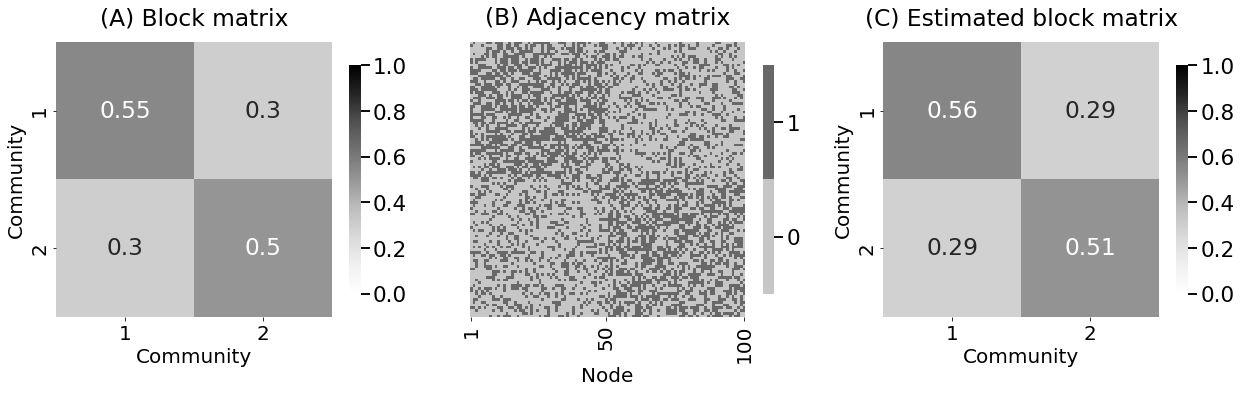
\includegraphics[width=\linewidth]{applications/ch7/Images/model_select_ex.png}
    \caption{\textbf{(A)} the true probability matrix underlying the $SBM_n(\vec z, B)$ random network, \textbf{(B)} a sample of the random network, \textbf{(C)} the estimated block matrix.}
    \label{fig:ch7:model:ex}
\end{figure}

\subsection{Model selection and random networks}

\textit{Model selection} is the task of selecting among several possible statistical models which we think may describe our sample. We do this using quantitative strategies to determine which statistical models are best supported by the data. 

\begin{floatingbox}[h]\caption{Model selection with coin flips}
\label{box:ch7:model:twosample_coin}
In Remark \ref{box:ch7:testing:twosample_coin}, we introduced a simple two-sample test for coin flip data. In this example, we wanted to determine whether the two coins had the same probability, or whether the probability was different. The null hypothesis was $H_0 : p_1 = p_2$, against $H_A : p_1 \neq p_2$. 

This example can also be thought of as a trivial example in model selection. In this case, we have two samples of data. While our question can be thought of as a two-sample test looking for a difference between the two samples, it can also be thought of as determining whether or not there were really two-samples of data in the first place.

Notice that under our null hypothesis, we are basically asking whether a coin with the same probability was used for both of the samples. Under the alternative hypothesis, we are basically asking whether two fundamentally different coins were used for each of the samples.

So, the null can be reformulated as: can the two samples be described using the same probability term, or can the two samples be best described using different probability terms. Stated another way, does the most reasonable model for the data have one parameter (the same probability term, for both samples), or should we describe it with two parameters (a unique probability term for each sample)?
\end{floatingbox}

In Remark \ref{box:ch7:model:twosample_coin}, we introduce the idea of model selection as it relates to a simple question of whether a collection of twenty coin flips (from two samples of data) should be described using a single probability term for all twenty coin flips, or whether each of the ten coin flips should be described using two probability terms.

In much the same light, we can formulate our block matrices under the same light. Remember that the block matrix for a simple $SBM_n(\vec z, B)$ random network is organized as:
\begin{align*}
    B &= \begin{bmatrix}
        b_{11} & b_{12} \\
        b_{12} & b_{22}
    \end{bmatrix}.
\end{align*}
The symmetry of $B$ is because the underlying simple random network is undirected (so $b_{21} = b_{12}$). What we want to do formally is ask, does the data provide us with enough evidence to support that the homophilic network is not a planted partition (does $b_{11} \neq b_{22}$)? Further, is there really any reason to believe that there is any block structure to it, at all?

If we only had the estimated block matrix in Figure \ref{fig:ch7:model:ex}(C), it feels immediate that we could conclude that the network is homophilic, but ``it feels immediate'' is not particularly quantitative.

As we move to more and more complicated models, there is concurrently a tradeoff known as model parsimony. \textit{Model parsimony} is the idea that simpler models with fewer parameters that describe are generally preferable to more complicated models with more parameters, provided both models describe the data equally well. This idea ties directly into the bias/variance tradeoff, which we discussed in Section \ref{sec:ch4:regularization}.

This can be interpreted with a level of rigor by considering the extremes. In the simplest case, we could have a random network model with a single parameter (an $ER_n(p)$ random network). On the other end of the spectrum, we have the most complicated model, which is an $IER_n(P)$ random network with a unique probability term $p_{ij}$ for each edge. 

The idea is that, with most datasets, we can find a ``happy medium'' somewhere in between, wherein the model is complicated enough that it describes our system faithfully, but not so complicated that we end up overfitting when we use our network sample to analyze it. Through model selection, we attempt to develop principled strategies that allow us to favor parsimonious models that are complicated enough to describe the data efficiently, but not so complicated that our data cannot support the downstream conclusions that we develop. 

\subsubsection*{Sequentially nested hypotheses}

A critical feature that we will exploit for model selection with $2 \times 2$ block matrices is the idea that we have nested hypotheses. A hypothesis $H_1$ is \textit{nested} in another hypothesis $H_2$ if, whenever $H_2$ is true, $H_1$ is true too. 

In the coin flip example, we can reformulate our two hypotheses $H_0$ and $H_A$ as a sequence of nested hypotheses. Notice that if $H_0$ is true, the model could be described with a single probability term $p_1 = p_2 = a$. On the other hand, if $H_A$ is true, the model can be described by $p_1 = b$ and $p_2 = c$. That $H_A$ is nested in $H_0$ would mean that even if we use two numbers $b$ and $c$ as the probabilities of $p_1$ and $p_2$, we could always just set $b = c$, and end up with the model in $H_0$. If in the underlying system it is the case that $p_1 \neq p_2$ (and $H_A$ is true), then we really need that additional delineation of terms $b$ and $c$. On the other hand, if in the underlying system it is the case that $p_1 = p_2$, we can get away with just the one term. 

\paragraph*{Developing sequentially nested hypotheses for network data}

To consider this idea of sequentially nested hypotheses for network data, let's think about the setting that we have with our $2 \times 2$ block matrix. In this case, we have three groups of edges: 
\begin{enumerate}
    \item the group of edges where both nodes are from community one,
    \item the group of edges where both nodes are from community two, and 
    \item the group of edges where one node is from community one and the other from community two.
\end{enumerate}
For each edge, we can build an edge group assignment matrix, which re-conceptualizes our $SBM_n(\vec z, B)$ random network as a $SIEM_n(D, \vec p)$ random network. We will still study the problem :

\begin{lstlisting}[style=python]
D = np.array(zs).reshape(n, 1) @ np.array(zs).reshape(1, n)
D[D == 4] = 3
\end{lstlisting}

This gives us three ``samples'' (to borrow the analogy from our coin flip model) of data. Visually, it seems pretty evident that the model is probably homophilic, so this motivates the following sequentially nested hypotheses:
\begin{enumerate}
    \item $H_0$: The block matrix is Erd\"os-R\'enyi, where $b_{11} = b_{12} = b_{22} = a$.
    \item $H_1$: The block matrix is a homophilic planted partition, where $b_{11} = b_{22} = a$, but $b_{12} = b$, and $a > b$. Note that this hypothesis is nested in $H_0$, as $H_0$ would be true if we were to choose $b$ where $a = b$.
    \item $H_2$: The block matrix is homophilic with heterogeneous on-diagonal blocks, where $b_{11} = a$, $b_{12} = b$, and $b_{22} = c$, where $b_{11}, b_{22} > b_{12}$. Note that this hypothesis is nested $H_1$, as $H_1$ would be true in a choice of $c$ where $a = c$.
\end{enumerate}


\paragraph*{Testing sequentially nested hypotheses}

The first question that you might have is how we can actually determine which of these sequentially nested hypotheses to pick. Remember that in the two hypothesis case, we tested the null hypothesis against the alternative hypothesis. In this case, however, we have three hypotheses, so we need a slightly different strategy. 

Since we already have strategies for testing two hypotheses, statisticians have come up with a simple but remarkably elegant solution to this problem. Basically, the idea is that we start with the simplest model that we could have ($H_0$). We add a single layer of complexity in the scope of the models that we think could be reasonable ($H_1$), and simply test $H_0$ as the null hypothesis against $H_1$ as the alternative hypothesis. 

Intuitively, the idea is that for a sequence of nested hypotheses with $N$ levels, for a hypothesis at level $n$ to be reasonable, then the hypothesis at level $n-1$ has to be more reasonable than the one at level $n-2$ first. In our case, this amounts to determining that if the model has a homophilic block matrix with a heterogeneous on-diagonal block structure, we should probably first know whether a homophilic block matrix makes sense in the first place. We basically follow this pattern backwards, which leads to the insight that it makes sense to begin at $H_0$ against $H_1$.

Once we test $H_0$ against $H_1$, we have two routes: either the data does not support $H_0$ and we reject $H_0$, or we do not have evidence to reject $H_0$. If we do not have evidence to reject $H_0$, we stop with the idea that we want to, in some sense, only move to complicated models when strictly necessary (e.g., when the data does not support the simpler model). We repeat this process over and over again, in the process known as \textit{forwards model selection}, in Algorithm \ref{alg:ch7:forwards}.

\begin{algorithm}[h]\caption{Forwards model selection}
\label{alg:ch7:forwards}
\KwData{$H_1, H_2, \hdots, H_N$ a sequence of sequentially nested hypotheses delineating different models to describe the data.}
\KwResult{The deepest hypothesis that is not rejected against the next sequential alternative.}
\SetAlgoLined

Set $n = 1$, and \texttt{stop=False}.

\While{\texttt{stop = False}} {
    
    Test $H_{n-1}$ as the null hypothesis against $H_n$ as the alternative hypothesis. 
    
    \uIf{no evidence to reject $H_{n-1}$\text{ or }$n = N - 1$} {
        Let \texttt{stop=True}.
    } \Else {
        Let $n = n + 1$.
    }
}

\Return{$H_n$}
\end{algorithm}

\subsection{Applying sequentially nested hypotheses to network data}

Remember with network data, the network samples have binary adjacency matrix entries $a_{ij}$ (which take values of $0$ or $1$). Remember that when we had two samples of data, a suitable representation was the contingency table in Table \ref{tab:ch7:testing:cont}. When we have three samples of binary data, what else can we use?

The best way to summarize this data is identical to that which we used for the two-class case: another contingency table. The contingency table for a $3$-sample example is lain out in Table \ref{tab:ch7:model:cont}.

\begin{table}[h]
    \centering
    \begin{tabular}{c | c|c|c}
         & Edge-group $1$ & Edge-group $2$ & Edge-group $3$ \\
         \hline
         Number of edges with $a_{ij} = 1$ & &  & \\
         Number of edges with $a_{ij} = 0$ & &  &
    \end{tabular}
    \caption{A contingency table with three samples.}
    \label{tab:ch7:model:cont}
\end{table}

In the two-sample case with $2$ columns, the Fisher's exact test is generally regarded as the preferred statistical test, however that only works with two samples (and not three). For this reason, we turn to the $\chi$-squared test, discussed briefly in Remark \ref{box:ch7:model:chisq}.

\begin{floatingbox}[h]\caption{The $\chi$-squared test for $2 \times K$ contingency tables}
\label{box:ch7:model:chisq}
When you have contingency tables with $K$ columns and $2$ rows, a good technique is known as the $\chi$-squared test. Unlike the Fisher's exact test, the $\chi$-squared test is an asymptotic test, in that it is effective when we have many samples of data, but has limitations when we do not have many samples of data. While it is generally preferable to defer to exact tests when possible, it will do for our purposes here. 

This statistical test gives us a test statistic, $X$, which is larger when the $K$ groups differ more, and small when the $K$ groups are the same. We use properties about the underlying network (that the edges are independent) to deduce what $X$ should look like if the $K$ groups are the same (known as the $\chi$-squared distribution). Finally, we obtain a $p$-value for our test by studying how anamalous the test statistic $X$ that we observed is compared to the $\chi$-squared distribution.
\end{floatingbox}

\begin{comment}
Without going into too much technical depth, the $\chi$-squared test operates on $2 \times K$ contingency tables and produces a number (the $\chi$-squared test statistic) which tends to be large when the $K$-way groupings differ, and tends to be small when the $K$-way groupings do not differ. 

This allows us to test whether, if $p_k$ are the column-wise mean probabilities for each of the $K$ levels, $H_0 : p_1 = p_2 = \hdots p_K$ against $H_A : p_k \neq p_l$ for some $k, l$. In words, it gives us a way to generalize the Fisher's exact test procedure to determine whether all of the columns have the same probability or whether some of the columns have different probabilities. 

Crucially, if we run two $\chi$-squared tests corresponding to two different table groupings with nested alternative hypotheses, we can compare the $\chi$-squared statistics (across the two different table groupings) and determine which grouping is more appropriate. 
\end{comment}

To refer back to our sequentially nested hypotheses, we can test whether the block model is Erd\"os-R\'enyi against whether it is homophilic planted partition directly, using the $2 \times 2$ contingency table in Table \ref{tab:ch7:model:cont_homo}. This produces a test statistic $X^{(1)}$, which we can use to test $H_0$ that the model is Erd\"os-R\'enyi against $H_A$ that the model is a homophilic planted partition. 

\begin{table}[h]
    \centering
    \begin{tabular}{c|c|c}
         & $(1, 1)$ and $(2, 2)$ blocks & $(1, 2)$ block \\
         \hline
         Number with $a_{ij} = 1$ & & \\
         Number with $a_{ij} = 0$ & & 
    \end{tabular}
    \caption{Contingency table for testing whether a block model is Erd\"os-R\'enyi against whether it is homophilic planted partition.}
    \label{tab:ch7:model:cont_homo}
\end{table}

In our data, the first step is to establish a model with the desired contingency table. We do this by using a \texttt{pandas} dataframe where the rows are edges, the firstcolumn indicates the value of the adjacency matrix for that particular edge, and the second column indicate the edge-group. Then, we indicate the \texttt{python} that we would like a statistical model for binary data by indicating a logistic regression with the \texttt{statsmodels} package:

\begin{lstlisting}[style=python]

\end{lstlisting}

Next, we run a second test, using the contingency table in Table \ref{tab:ch7:model:cont_het}. This produces a test statistic $X^{(2)}$, which we can use to test $H_0$ that the model is not homophilic with heterogeneous on-diagonal blocks against $H_A$ that the model is homophilic with heterogeneous on-diagonal blocks. 

\begin{table}[h]
    \centering
    \begin{tabular}{c|c|c|c}
         & $(1, 1)$ block & $(1, 2)$ block & $(2, 2)$ block \\
         \hline
         Number with $a_{ij} = 1$ & & & \\
         Number with $a_{ij} = 0$ & & & 
    \end{tabular}
    \caption{Contingency table for testing whether a block model is Erd\"os-R\'enyi against whether it is homophilic planted partition.}
    \label{tab:ch7:model:cont_het}
\end{table}

The magic occurs here: when we look at the ratio $\frac{X^{(2)}}{X^{(1)}}$, the test that we are really running when the hypotheses are sequentially nested is a test of whether $H_0$ the model is a homophilic planted partition against $H_A$ that the model is homophilic with heterogeneous on-diagonal blocks. This strange result occurs because, when the hypotheses are nested, we can describe what $\frac{X^{(2)}}{X^{(1)}}$ looks like if the more complicated model does not add any value to the simpler model. Whereas the reference before was the $\chi$-squared distribution, the reference here is known as the $F$-distribution. 

This procedure is generally known as an \textit{Analysis of Variance} (ANOVA), and is extremely common when comparing $K$ groups of data in both binary and non-binary situations. In our case, our network samples have adjacency matrix entries with binary values ($0$ or $1$), so we can use it.

\begin{lstlisting}[style=python]

\end{lstlisting}

\newpage